%%
%% This is file `sample-sigconf.tex',
%% generated with the docstrip utility.
%%
%% The original source files were:
%%
%% samples.dtx  (with options: `sigconf')
%% 
%% IMPORTANT NOTICE:
%% 
%% For the copyright see the source file.
%% 
%% Any modified versions of this file must be renamed
%% with new filenames distinct from sample-sigconf.tex.
%% 
%% For distribution of the original source see the terms
%% for copying and modification in the file samples.dtx.
%% 
%% This generated file may be distributed as long as the
%% original source files, as listed above, are part of the
%% same distribution. (The sources need not necessarily be
%% in the same archive or directory.)
%%
%% The first command in your LaTeX source must be the \documentclass command.
\documentclass[manuscript]{acmart} %need to change [manuscript]
\newcommand{\squeezeup}{\vspace{-6mm}}
\newcommand{\squeezeuplittle}{\vspace{-3pt}}
\newcommand{\squeezeuphalf}{\vspace{-2mm}}
%% NOTE that a single column version is required for 
%% submission and peer review. This can be done by changing
%% the \doucmentclass[...]{acmart} in this template to 
%% \documentclass[manuscript,screen]{acmart}
%% 
%% To ensure 100% compatibility, please check the white list of
%% approved LaTeX packages to be used with the Master Article Template at
%% https://www.acm.org/publications/taps/whitelist-of-latex-packages 
%% before creating your document. The white list page provides 
%% information on how to submit additional LaTeX packages for 
%% review and adoption.
%% Fonts used in the template cannot be substituted; margin 
%% adjustments are not allowed.

%%
%% \BibTeX command to typeset BibTeX logo in the docs
\AtBeginDocument{%
  \providecommand\BibTeX{{%
    \normalfont B\kern-0.5em{\scshape i\kern-0.25em b}\kern-0.8em\TeX}}}

%% Rights management information.  This information is sent to you
%% when you complete the rights form.  These commands have SAMPLE
%% values in them; it is your responsibility as an author to replace
%% the commands and values with those provided to you when you
%% complete the rights form.
%%\setcopyright{acmcopyright}
%%\copyrightyear{2021}
%%\acmYear{2021}
%%\acmDOI{}

%% These commands are for a PROCEEDINGS abstract or paper.
%%\acmConference[SA '21]{SA ’21 Emerging Technologies}{December 14-17, 2021}{Tokyo, Japan}
%%\acmBooktitle{SA '21:  SIGGRAPH Asia 2021 Emerging Technologies (SA ’21 Emerging Technologies),
%%  December 14-17, 2021, Tokyo, Japan}
%%\acmPrice{15.00}
%%\acmISBN{}

\setcopyright{rightsretained}
\copyrightyear{2024}
\acmYear{2024}
\acmConference{(SIGGRAPH '24 Immersive Pavilion:}{July 28 - August 1, 2024}{Denver,
United States of America}
\acmBooktitle{SIGGRAPH 2024 Immersive Pavilion (SIGGRAPH '24 Immersive Pavilion),July 28 - August 1, 2024}
\acmDOI{10.1145/3476122.3484837}
\acmISBN{978-1-4503-8685-2/21/12}

%%
%% Submission ID.
%% Use this when submitting an article to a sponsored event. You'll
%% receive a unique submission ID from the organizers
%% of the event, and this ID should be used as the parameter to this command.
%%\acmSubmissionID{123-A56-BU3}

%%
%% The majority of ACM publications use numbered citations and
%% references.  The command \citestyle{authoryear} switches to the
%% "author year" style.
%%
%% If you are preparing content for an event
%% sponsored by ACM SIGGRAPH, you must use the "author year" style of
%% citations and references.
%% Uncommenting
%% the next command will enable that style.
\citestyle{acmauthoryear}

%%
%% end of the preamble, start of the body of the document source.
\begin{document}


%%
%% The "title" command has an optional parameter,
%% allowing the author to define a "short title" to be used in page headers.
\title{ColabSurgVR: A Virtual Reality Surgical Planning and Collaborative Platform}

%Imports bibliography file
%%
%% The "author" command and its associated commands are used to define
%% the authors and their affiliations.
%% Of note is the shared affiliation of the first two authors, and the
%% "authornote" and "authornotemark" commands
%% used to denote shared contribution to the research.

\author{Jing-Yuan Huang}
\affiliation{%
  \institution{National Taiwan University}
  %\city{Taipei}
  \country{Taipei, Taiwan}
}

%%
%% By default, the full list of authors will be used in the page
%% headers. Often, this list is too long, and will overlap
%% other information printed in the page headers. This command allows
%% the author to define a more concise list
%% of authors' names for this purpose.
\renewcommand{\shortauthors}{Jing-Yuan Huang, et al.}

%%
%% The abstract is a short summary of the work to be presented in the
%% article.
\begin{abstract}

\vspace{-0.45em}
\end{abstract}



%%
%% The code below is generated by the tool at http://dl.acm.org/ccs.cfm.
%% Please copy and paste the code instead of the example below.
%%
\begin{CCSXML}
<ccs2012>
 <concept>
  <concept_id>10010520.10010553.10010562</concept_id>
  <concept_desc>Computer systems organization~Embedded systems</concept_desc>
  <concept_significance>500</concept_significance>
 </concept>
 <concept>
  <concept_id>10010520.10010575.10010755</concept_id>
  <concept_desc>Computer systems organization~Redundancy</concept_desc>
  <concept_significance>300</concept_significance>
 </concept>
 <concept>
  <concept_id>10010520.10010553.10010554</concept_id>
  <concept_desc>Computer systems organization~Robotics</concept_desc>
  <concept_significance>100</concept_significance>
 </concept>
 <concept>
  <concept_id>10003033.10003083.10003095</concept_id>
  <concept_desc>Networks~Network reliability</concept_desc>
  <concept_significance>100</concept_significance>
 </concept>
</ccs2012>
\end{CCSXML}

\ccsdesc[500]{Human-centered computing~Interaction paradigms}
\ccsdesc{Human-centered computing~Virtual Realty}
%%
%% Keywords. The author(s) should pick words that accurately describe
%% the work being presented. Separate the keywords with commas.
\keywords{Preoperative Planning, 3D Visualization, Surgical Collaboration, Virtual Reality}

%% A "teaser" image appears between the author and affiliation
%% information and the body of the document, and typically spans the
%% page.
\begin{teaserfigure}
  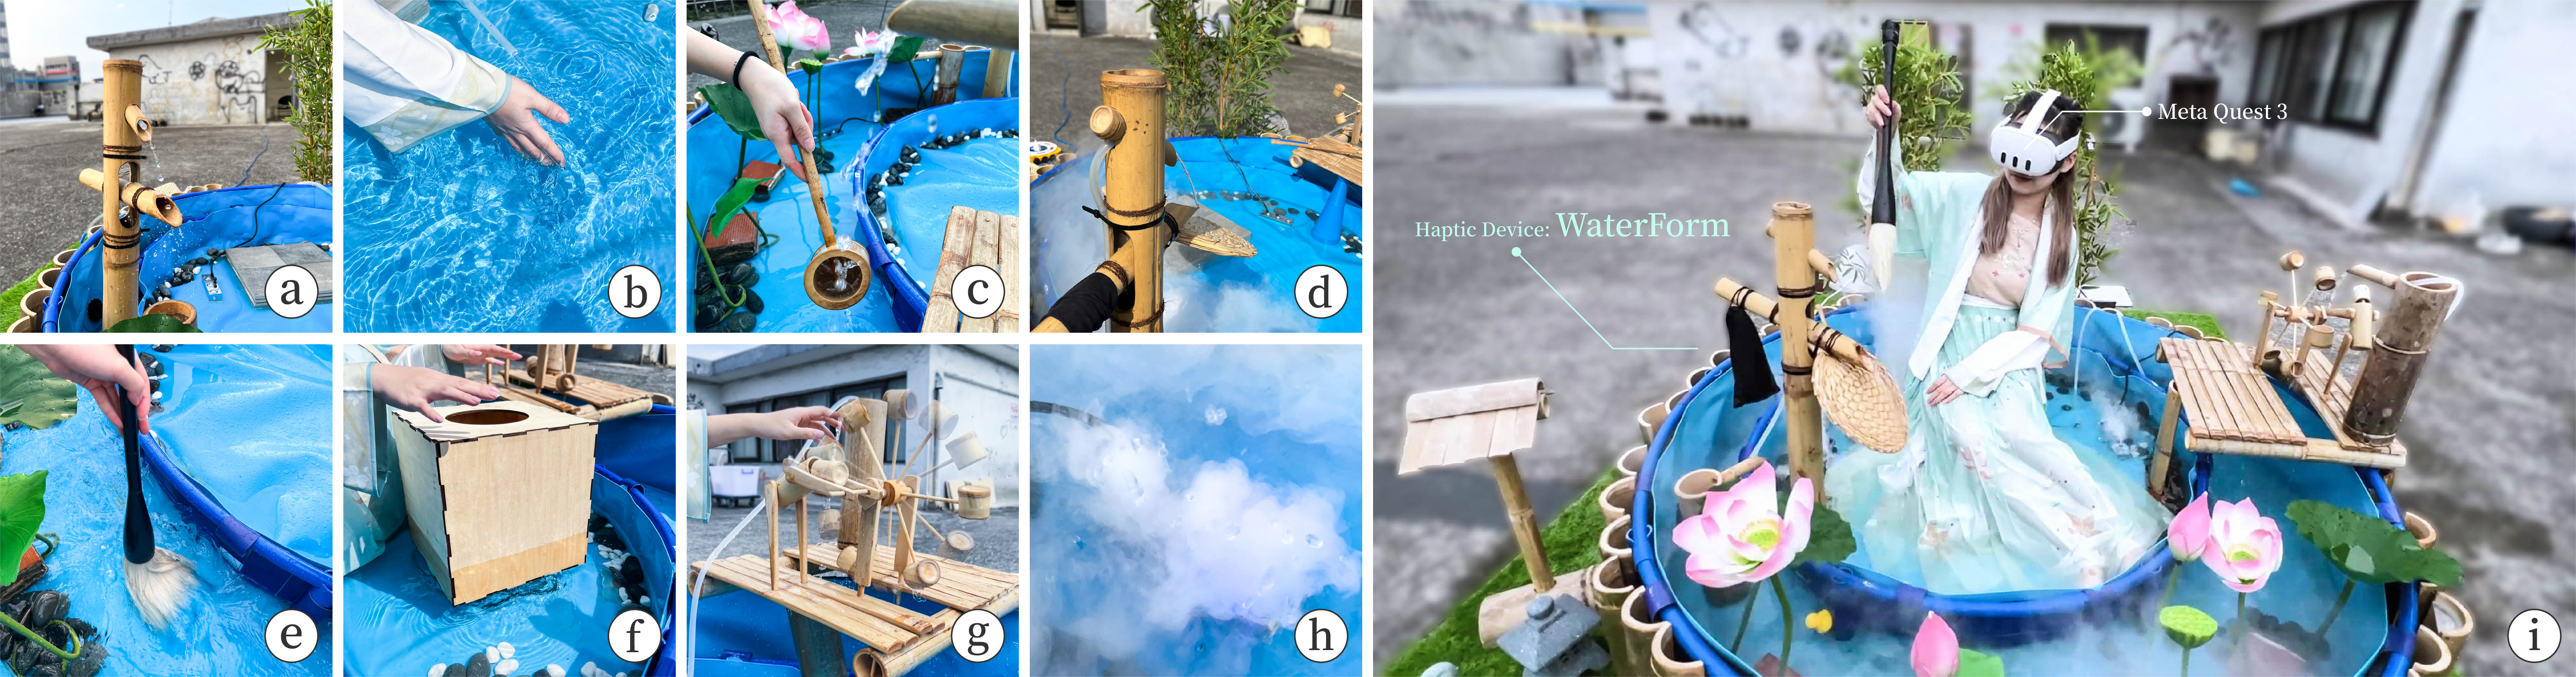
\includegraphics[width=\textwidth]{WF_SA.png}
  \vspace{-1.75em}
  \caption{Our Liquid-transformation Systems produces (a) water splash, (b) water flow, (c) gravity, (d) wind,  (e) resistance, (f) buoyant force, (g) mechanical energy, and (h) mist to enhance (i) immersive environment.}
  \vspace{0.5em}
  \Description{}
  \label{fig:teaser}
\end{teaserfigure}

%%
%% This command processes the author and affiliation and title
%% information and builds the first part of the formatted document.
\maketitle

\section{INTRODUCTION}

Accurate visuospatial conversion of 2D medical images into 3D mental models is essential in clinical practice. However, such skills are challenging to acquire and require significant cognitive effort, especially for novice medical practitioners. Immersive 3D visualizations of surigcal amaotmy in Virtual reality (VR) have been explored to facilitate visuospatial udnerstanding, preoperative planning, and interprofessional collaboration. \cite{RN86} developed a 3D heart model for medical education in a semi-immersive environment with navigational tools. \cite{RN5} demonstrated that 3D-VR is a valid tool for teaching surgical anatomy in unique patient case and adds more enjoyment to the learning process. LapSim \cite{RN90} provided a realistic stimulation for thoracoscopic surgeries and especially benefited the novices without prior experience. In the context of patient-specific preoperative evaluation, \cite{RN83} proposed an immersive presentation of medical volume data for liver surgery planning. CollaVRLap \cite{RN26} additionally implemented the co-presence of an assistant to stimulate for cooperation in laparoscopic liver surgery training. \cite{RN6} further delinated a VR environment focusing on collaborative virtual resection for liver surgery, either in remote or co-located environment. For thoracic anatomy, PulmoVR \cite{RN10, RN13} combined VR with semi-automatic segmentation for immersive planning of lung surgeries, and demonstrated clinical benefits in optimizing surgical plans. Similarly, \cite{RN44} showcased the improvements in understading and planning accuracy provided by VR for residents surgeons.
%VisCubeSX \cite{RN85} improved the resident knowledge of pelvic anatomy compared to traditional methods.
% Ujiie et al. (2021) developed a VR simulation system for thoracic surgery, emphasizing its utility in preoperative planning and intraoperative assistance. 
%Elucis \cite{RN84} validated a VR platform for 3D anatomical modeling and contouring in radiation oncology and surgical planning, showing substantial efficiency improvements and high similarity to existing commercial platforms. 
%Kunz et al. (2024) assessed the use of VR for understanding and evaluating anatomical data in pancreatic cancer resectability, highlighting the potential for more accurate staging of pancreatic ductal adenocarcinoma.

Despite these advancements, current VR systems face several gaps and limitations, including inadequate interaction capabilities, limited visualization of patient data, and insufficient support for collaborative planning among multidisciplinary teams. Additionally, there is a need for high-fidelity 3D models in real-time, interactive environments to facilitate comprehensive surgical planning, and thorough validation is required to ensure their effectiveness in clinical applications. To address these issues, this paper presents a novel VR surgical planning system designed to enhance preoperative planning accuracy and efficiency through immersive 3D visualizations of patient-specific anatomy. The system supports real-time, interactive collaboration among multidisciplinary teams and involves semi-automatic segmentation and manual refinement to generate high-fidelity 3D models, optimized using mesh processing techniques. Initial validation through a pilot study demonstrated the system’s functional accuracy and potential to improve surgical outcomes.


%\vspace{-0.5em}
\section{DESIGN AND IMPLEMENTATION}


\section{APPLICATION}


\section{DISCUSSION AND FUTURE WORK}


%%
%% The next two lines define the bibliography style to be used, and
%% the bibliography file.
\bibliographystyle{ACM-Reference-Format}
\bibliography{sample-base}

%%
%% If your work has an appendix, this is the place to put it.
\appendix

\end{document}
\endinput
%%
%% End of file `sample-sigconf.tex'.